\def \t#1{t$_#1$}

\section{Experiments and Evaluations}
\label{sect:exper}

In this section, we introduce the experiments conducted on two datasets for
evaluating the performance of our implementations. We report the experiment
results and present our observations and perceptives based on the results.





% --------------------------------------------------
\subsection{Experimental Setting}

We have conducted several experiments to evaluate the performance of our
implementations of parallel XPath queries. All the experiments were conducted on
a computer that equipped with two Intel Xeon E5-2620 v3 CPUs (6 cores, 2.4GHz,
Hyper-Threading off) and 32-GB memory (DDR4-1866). Software we used ware Java
OpenJDK ver. 9-internal (64-Bit Server VM) and BaseX ver. 8.6.4 with minor
modifications to enable TCP\textunderscore NODELAY, which is
used to improve tcp/ip networks and decrease the number of packets.

We used two larege XML documents for the experiments: \texttt{xmark10.xml} and
\texttt{dblp.xml}. The dataset \texttt{xmark10.xml} is an XMark
dataset~\cite{XMark} generated with the parameter 10, which was of 1.1 GB and
had 16 million nodes. The root of the XMark tree has six children
\verb|regions|, \verb|people|, \verb|open_auctions|, \verb|closed_auctions|,
\verb|catgraph|, and \verb|categories|, which have 6, 255000, 120000, 97500,
10000, and 10000 children, respectively. The dataset \texttt{dblp.xml} was
downloaded on Febrary 13, 2017 from~\cite{DBLP}, which is an open bibliographic
information database on major computer science journals and proceedings. It
sizes 1.85 GB and has 46 million nodes. The root has 5.5 million nodes of eight
different names, including  \texttt{article},  \texttt{book},
\texttt{incollections},  \texttt{inproceedings},  \texttt{masterthesis},
\texttt{phdthesis}, \texttt{proceedings},  \texttt{www}.


We used the XPath queries shown in Table~\ref{tab:dpsqueries} for data
partitioning and Table~\ref{tab:qpsqueries} for query partitioning, which are
the same as those used in~\cite{BoLS09}, and measured execution times until we
obtained the whole serialized string as the result. The execution time does not
include the loading time, that is, the input XML tree was loaded into memory
before the execution of queries. To reduce the effect of fluctuations, we
measured execution time for 51 times, and calculated their average after
removing top-10 and bottom-10 results.


% --------------------------------------------------
\subsection{Evaluation on Implementations of Data Partitioning Strategy}

In this section, we evaluate two of our implementations of data partitioning
strategy. We also analysis the speedup and scalability of them.

\subsubsection{Total Execution Time}

\begin{table}[tbp]
\caption{Summary of execution time of data partitioning}
\label{Table:summary}
\small
\setlength{\doublerulesep}{.4pt}
\centering\begin{tabular}{l|c|rr@{~(}r@{)}|rr@{~(}r@{)}|rr}
\hline \hline
~~Key & orig $t_o$~ & \multicolumn{3}{c|}{client-side} & \multicolumn{3}{c|}{server-side} & \multicolumn{2}{c}{Result size} \\
	&       			& seq $t_s$~   	& par $t_p$~   	& $t_o/t_p$	& seq $t_s$~	& par $t_p$~	& $t_o/t_p$	& prefix~	& final~ \\
\hline
XM1(a)	& 25796.64			& 27916.83	& 12392.80	& 2.08		& 28161.89	& 11484.99	& 2.25		& 54		& 994 M \\
\hline
XM2(a)	& \multirow{3}{*}{1.33}		& 2996.85	& 959.18	& 0.00		& 1159.78	& 760.62	& 0.00		& 6.62 M	& \multirow{3}{*}{1.55 K} \\
XM2(b)	&				& 1018.59	& 707.38	& 0.00		& 894.94	& 529.75	& 0.00		& 54		&  \\
XM2(c)	&				& 3.43		& 4.56		& 0.29		& 5.29		& 6.26		& 0.21		& 671		&  \\
\hline
XM3(a)	& \multirow{3}{*}{595.75}	& 900.69	& 297.88	& 2.00		& 706.95	& 226.54	& 2.63		& 1.08 M	& \multirow{3}{*}{14.5 M} \\
XM3(b)	&				& 1519.92	& 1148.42	& 0.52		& 1472.53	& 987.48	& 0.60		& 54		&  \\
XM3(c)	&				& 1029.85	& 308.67	& 1.93		& 723.44	& 297.31	& 2.00		& 1.08 M	&  \\
\hline
XM4(a)	& \multirow{3}{*}{798.16}	& 1290.36	& 699.99	& 1.14		& 1241.34	& 559.32	& 1.43		& 49		& \multirow{3}{*}{26.4 M} \\
XM4(b)	&				& 1786.89	& 564.82	& 1.41		& 1216.57	& 406.93	& 1.96		& 1.75 M	&  \\
XM4(c)	&				& 929.37	& 204.69	& 3.90		& 872.97	& 209.72	& 3.81		& 106 K		&  \\
\hline
XM5(a)	& \multirow{2}{*}{659.76}	& 2311.56	& 751.65	& 0.88		& 1212.33	& 564.28	& 1.17		& 5.38 M	& \multirow{2}{*}{15.9 M} \\
XM5(b)	&				& 1018.26	& 500.98	& 1.32		& 832.28	& 501.04	& 1.32		& 1.08 M	&  \\
\hline
XM6(a)	& \multirow{2}{*}{790.99}	& 811.57	& 639.59	& 1.24		& 825.20	& 661.54	& 1.20		& 49		& \multirow{2}{*}{22.2 M} \\
XM6(b)	&				& 875.33	& 189.20	& 4.18		& 810.15	& 190.67	& 4.15		& 183 K		&  \\
\hline
DBLP1(a) & 3797.36 & 9138.82  & 2219.10 & 1.71    & 6152.72  & 1895.17 & 2.00    & 13.2 MB & 133 MB \\ 
\hline
DBLP2(a) & 9684.71 & 29389.93 & 9473.94 & 1.02    & 12789.19 & 5718.26 & 1.69    & 47.0 MB & 356 MB \\ 
\hline
\end{tabular}
\end{table}


Table~\ref{Table:summary} summarizes the execution times of the queries. The
``orig $t_o$''column shows the time for executing original queries XM1--XM6 and
DBLP1--DBLP2 with BaseX's \verb|xquery| command. The ``seq $t_s$'' columns show
the time for executing the prefix query and the suffix query with a single
thread. The ``par $t_p$'' columns show the time for executing the prefix query
with one thread and the suffix query with 12 threads (6 threads for XM1(a) and 8
threads for DBLP2(a)).  The table also includes for reference the speedup of
parallel queries with respect to original queries and the size of results of the
prefix queries and the whole queries.

By using the pair of the prefix and suffix queries split at an appropriate step,
we obtained speedups of factor two for XM1 and XM3, and factor of more than 3.5
for XM4 and XM6. The original execution time of XM2 was very short since BaseX
executed an optimized query that utilized an index over attributes. By designing
the parallel query XM2(c) based on that optimized query, the execution time of
parallel query was just longer than that of original query by 5 ms. For the
DBLP1(a) and DBLP2(b), the speedups are 1.71 and 1.02 on the client-side, while
2.00 and  1.69 on the server-side. Comparing the client-side and server-side
implementation, we observed that the server-side implementation ran faster for
most queries and performance differences were merely within the fluctuations
even for the exceptions.

\subsubsection{Breakdown of Execution Time}

\begin{table}[tbp]
\caption{Breakdown of execution time for client-side implementation}
\label{table:breakdown-c}
\small
\setlength{\doublerulesep}{.4pt}
\centering\begin{tabular}{l|r|rrrrr@{~~(}c@{)}|r}
\hline
\hline
Key     & prefix        & \multicolumn{6}{c|}{suffix \raisebox{-.7pt}{$t^P$}}                                                   		& merge\\
	& 		& \makebox[4.2em][c]{P=1}	& \makebox[4.2em][c]{P=2}	& \makebox[4.2em][c]{P=3}	& \makebox[4.2em][c]{P=6}	& \makebox[4.2em][c]{P=12} & $t^{1}/t^{12}$ & \\
\hline
XM1(a)	& 4.63		& 27569.07	& 20756.44	& 20270.44	& 11758.00	&		& 2.34		& 287.08 \\
XM3(c)	& 66.57		& 938.62	& 505.57	& 376.84	& 259.64	& 229.03	& 4.10		& 6.34 \\
XM4(c)	& 14.64		& 895.02	& 550.90	& 399.07	& 215.49	& 172.66	& 5.18		& 9.12 \\
XM5(b)	& 68.24		& 927.22	& 668.38	& 533.90	& 452.73	& 424.29	& 2.19		& 3.70 \\
XM6(b)	& 17.00		& 842.94	& 488.21	& 360.93	& 194.28	& 157.65	& 5.35		& 8.17 \\
DBLP1(a) & 772.518  & 8412.663 & 5358.734 & 3512.645 & 2017.838 & 1413.355 & 5.95   & 33.222  \\ 
DBLP2(a) & 2006.868 & 29261.43 & 17381.72 & 12747    & 7843.271 & 7194.168 & 4.07   & 272.906 \\ \hline
\end{tabular}
\end{table}

\begin{table}[tbp]
\caption{Breakdown of execution time for server-side implementation}
\label{table:breakdown-s}
\small
\setlength{\doublerulesep}{.4pt}
\centering\begin{tabular}{l|r|rrrrr@{~~(}c@{)}|r}
\hline
\hline
Key  & prefix        & \multicolumn{6}{c|}{suffix \raisebox{-.7pt}{$t^P$}}                                                   		& merge\\
	& 		& \makebox[4.2em][c]{P=1}	& \makebox[4.2em][c]{P=2}	& \makebox[4.2em][c]{P=3}	& \makebox[4.2em][c]{P=6}	& \makebox[4.2em][c]{P=12} & $t^{1}/t^{12}$ & \\
\hline
XM1(a)	&  5.09		& 27798.44	& 21155.57	& 20121.32	& 11047.99	&		& 2.52		& 192.27 \\
XM3(c)	& 72.34		& 631.65	& 380.00	& 284.87	& 202.25	& 210.98	& 2.99		&   3.43 \\
XM4(c)	& 16.20		& 840.24	& 530.57	& 376.44	& 198.55	& 170.17	& 4.94		&  10.46 \\
XM5(b)	& 65.27		& 744.58	& 526.82	& 435.24	& 407.45	& 423.56	& 1.76		&   4.99 \\
XM6(b)	& 17.22		& 776.99	& 450.99	& 323.49	& 176.92	& 157.47	& 4.93		&   5.98 \\
\hline
DBLP1(a) & 814.872  & 5298.603 & 2954.788 & 2092.14  & 1245.178 & 1039.821 & 5.10   & 40.475  \\ 
DBLP2(a) & 1911.724 & 13437.98 & 9223.007 & 6787.181 & 3812.572 & 3459.338 & 3.88   & 347.2   \\ 
\hline
\end{tabular}
\end{table}


To investigate the execution time in detail, we executed parallel queries
XM1(a), XM3(c), XM4(c), XM5(b), XM6(b) DBLP(a) and DBLP(a) with $P=1$, 2, 3, 6,
and 12 threads. Tables~\ref{table:breakdown-c} and \ref{table:breakdown-s} show
the breakdown of the execution time divided into three phases: prefix query,
suffix query and merge. In these tables, the speedup is calculated with respect
to the execution time of suffix queries with one thread.

From Tables~\ref{table:breakdown-c} and \ref{table:breakdown-s} we can find
several interesting observations. First, the execution time of prefix queries
was almost proportional to their result sizes and almost the same between the
two implementations. Comparing the two implementations, we can observe that the
server-side implementation outperformed the client-side implementation in all
suffix queries, where differences in merge were by definition within the
fluctuations.  These results suffice for concluding that the server-side
implementation is, as expected, more efficient.

Next, we analyze the dominant factor of the performance gaps between the
client-side and the server-side implementations. Although the performance gaps
of prefix queries should be mainly the difference between sending data to
clients on localhost and storing data into memory, it was not significant.
Communication cost, which is our expected advantage of the server-side
implementation, therefore did not explain the dominant factor of total
performance gaps.

By examining the logs of the BaseX server, we have found that the dominant
factor was parsing of suffix queries. Since the client-side implementation sends
a suffix query of length linearly proportional to the result size of a prefix
query, it can be long. In fact, the suffix query of XM3(c) for the 1-thread case
was 1.1 MB and BaseX took 141.82 ms for parsing the query string. Sending and
receiving a long query per se would not cost so much because localhost
communication and local memory access were not so different in performance.
Parsing is, however, more than sequential memory read like deserialization that
the server-side does. Parsing is essentially not streamable. Before finishing
parsing a query, BaseX cannot start to evaluate it, whereas the deserialization
in the server-side is streamable. We conclude that this difference in
streamability was the dominant factor of the performance gaps between the
client-side and the server-side.

For the DBLP queries, apart from the results that follow the observations from
XM queries, We also notice that BaseX did not apply optimization on the
descendant axis in DBLP2, which is caused by the structure of \texttt{dblp}
dataset, which has 5515443 child nodes of eight unique names: \texttt{article,
book, incollections, inproceedings, masterthesis, phdthesis, proceedings, www}.
Every child of the root \texttt{dblp} represents a publication that has the
information such as \texttt{title}, \texttt{author}, \texttt{year} etc. Since
the paths are different (from example, a \texttt{title} could on the path of
\texttt{/dblp/article/title} or \texttt{/dblp/book/title}), BaseX cannot apply
the optimization that replaces descendant axis with the same child axes to all
the matching nodes of \texttt{title}. In this case, query partitioning is useful
to improve the query performance. We discuss this in Section~\ref{sec:qpseval}.

\subsubsection{Scalability Analysis}
\label{sec:dpsscal}

When we analyze the speedup of parallel execution, the ratio of sequential
execution part to the whole computation is important because it limits the
possible speedup by Amdahl's law. In the two implementations, the sequential
execution part consists of the prefix query and merge. The ratio of the
sequential execution part was small in general: more specifically, the
client-side implementation had smaller ratio (less than 7\%) than the
server-side implementation had (less than 10\%). In our implementation, the
suffix queries were executed independently in parallel through individual
connections to the BaseX server. The speedups we observed for the suffix queries
were, however, smaller than we had expected.  We also noticed that in some cases
the execution time was longer with 12 threads than with 6 threads (for example,
XM5(b) with the server-side implementation).

To understand the reason why the speedups of the suffix queries were small, we
made two more analyses. Figure \ref{fig:load-balance} plots the degree of load
balance of the suffix query, calculated as the sum of execution times divided
the maximum of execution times. The degree of load balance is defined as $\sum
t_i^{p} / \max t_i^p$, where $t_i^p$ denotes the execution time of the $i$th
suffix query in parallel with $p$ threads. Figure \ref{fig:increase-of-work}
plots the increase of work of the suffix queries, calculated by the sum of
execution times divided by that of one thread. The increase of work is defined
as $\sum t_i^{p} / t_1^{1}$.

From Figs~\ref{fig:load-balance} and ~\ref{fig:increase-of-work}, we can observe
the reasons of the small speedups in the suffix queries. First, when the prefix
query returned a very small number of results (as for XM1(a)), the load of
suffix queries was ill balanced. This was the main cause that the query XM1(a)
had small speedups in the suffix queries. For the other cases, we achieved good
load-balance until 6 threads, and the degrees of load-balance were more than
83\% even with 12 threads, which means that load ill-balance was not the main
cause of small speedups for those queries. Secondly, the increase of work was
significant for XM5(b) and XM3(c), and it was the main cause that the queries
XM5(b) and XM3(c) had small speedups. For the other queries, we observed almost
no increase of work until 6 threads, but the work increased when 12 threads.
Such an increase of work is often caused by contention to memory access, and it
is inevitable in shared-memory multicore computers.

\begin{figure}[t]
 \begin{minipage}{.48\linewidth}
  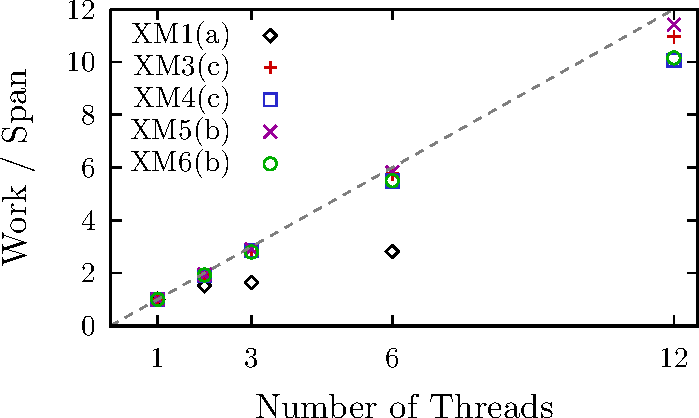
\includegraphics[width=.98\linewidth]{basex/exp_results/load_balance.pdf}
  \caption{Load balance}
  \label{fig:load-balance}
 \end{minipage}
 \hfill
 \begin{minipage}{.48\linewidth}
  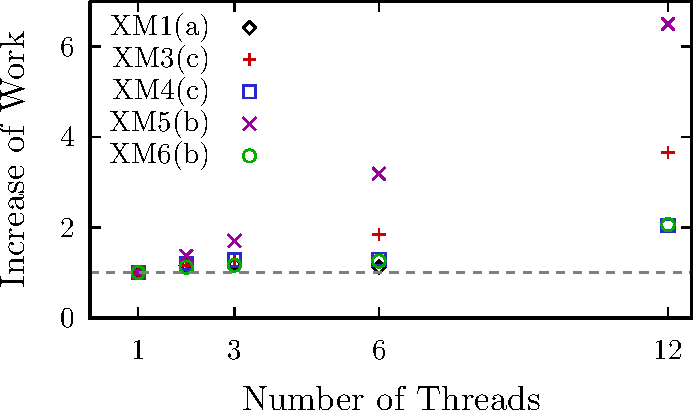
\includegraphics[width=.98\linewidth]{basex/exp_results/increase_of_work.pdf}
  \caption{Increase of work}
  \label{fig:increase-of-work}
 \end{minipage}
\end{figure}

% --------------------------------------------------
\subsection{Evaluation on Implementation of Query Partitioning Strategy}
\label{sec:qpseval}

Table~\ref{tab:qpstotaltime} summarizes the total execution time of the queries.
The ``orig \t{o}'' column shows the time for executing original queries XM1--XM6
and DBLP1--DBLP2 with BaseX's \texttt{xquery} command. The ``seq \t{s}'' columns
show the time for executing all the subquery one by one with a single thread.
The ``par \t{p}'' columns show  the time for executing the x query with one
thread and the with 12 or 6 threads depending on queries. The table also
includes reference of the speedup of parallel queries with respect to original
queries and the size of results of the original queries.


\begin{table}[t]
\centering
\caption{Summary of total execution times(ms) of queries by query partitioning}
\label{tab:qpstotaltime}
	\begin{tabular}{c|c|c|c|c|c}
		\hline
		\multirow{2}{*}{Key} & \multirow{2}{*}{orig \t{o}}  & \multicolumn{3}{c|}{Implementation of Query Partitioning} & Result size             \\ \cline{3-6}
		&                           & seq \t{s}             & par \t{p}             & \t{o}/\t{p}          & Final                   \\ \hline
		XM1(d)               & \multirow{2}{*}{25796.64} & 25326.472           & 11624.09           & 2.22           & \multirow{2}{*}{994M}   \\ \cline{1-1} \cline{3-5}
		XM1(e)               &                           & 31561.45            & 11514.87           & 2.24           &                         \\ \hline
		XM2(d)               & \multirow{2}{*}{1.33}     & 362.564             & 415.38             & 0.00           & \multirow{2}{*}{1.55 K} \\ \cline{1-1} \cline{3-5}
		XM2(e)               &                           & 4.05                & 1.26               & 1.06           &                         \\ \hline
		XM3(d)               & 595.75                    & 754.439             & 146.64             & 4.06           & 14.5 M                  \\ \hline
		XM4(d)               & \multirow{2}{*}{798.16}   & 1098.432            & 516.98             & 1.54           & \multirow{2}{*}{26.4 M} \\ \cline{1-1} \cline{3-5}
		XM4(e)               &                           & 1163.919            & 523.62             & 1.52           &                         \\ \hline
		XM5(d)               & \multirow{2}{*}{659.76}   & 869.089             & 288.21             & 2.29           & \multirow{2}{*}{15.9 M} \\ \cline{1-1} \cline{3-5}
		XM5(e)               &                           & 1536.161            & 1031.46            & 0.64           &                         \\ \hline
		XM6(d)               & \multirow{2}{*}{790.99}   & 744.873             & 646.67             & 1.22           & \multirow{2}{*}{22.2 M} \\ \cline{1-1} \cline{3-5}
		XM6(e)               &                           & 739.449             & 640.57             & 1.23           &                         \\ \hline
		DBLP1                & 3797.36                   & 6572.87             & 1618.51            & 2.35           & 133 M                   \\ \hline
    DBLP2                & 9684.71                   & 12524.70            & 6160.54            & 1.57           & 356 M                   \\ \hline
	\end{tabular}
    \vspace{10px}
	\centering
\caption{Breakdown of execution time (ms)}
\label{tab:qpsbreakdown}
\begin{tabular}{c|c|c|c|c|c|c|c}
	\hline
	\multirow{2}{*}{Key} & \multicolumn{6}{c|}{Subqueries}                              & \multirow{2}{*}{Merge} \\ \cline{2-7}
	& P=1      & P=2      & P=3      & P=6      & P=12    & t$^1$/t$^{12}$ &                        \\ \hline
	XM1(d)               & 25606.42 & 18583.66 & 18701.76 & 11420.36 &         & 2.24   & 203.73                 \\ \hline
	XM2(d)               & 356.67   & 384.08   & 367.99   & 345.89   & 415.38  & 0.86   & 0.00                   \\ \hline
	XM3(d)               & 540.14   & 327.03   & 241.33   & 159.63   & 141.82  & 3.81   & 4.82                   \\ \hline
	XM4(d)               & 897.38   & 786.46   & 550.56   & 507.15   &         & 1.77   & 9.83                   \\ \hline
	XM5(d)               & 670.15   & 415.35   & 314.01   & 284.40   & 282.14  & 2.38   & 6.07                   \\ \hline
	XM5(e)               & 701.94   & 698.77   & 735.18   & 828.65   & 1025.09 & 0.68   & 6.37                   \\ \hline
	XM6(d)               & 789.65   & 799.93   & 790.82   & 636.41   &         & 1.24   & 10.26                  \\ \hline
	DBLP1(d)             & 4035.83  & 2609.61  & 1931.22  & 1567.33  & 1584.97 & 2.55   & 33.53                  \\ \hline
\end{tabular}
\end{table}


\subsubsection{Total Execution Times and Speedups}

From Table~\ref{tab:qpstotaltime}, we can see that for most of the queries we
have obtained speedups of factors  more than 1 and XM3(d) obtains the most
speedup of a factor of 4.06. This means that we can accelerate the execution by
query partitioning for these queries. We also notice that there are two queries,
on the contrary, which have been decelerated: XM2(d) and XM5(e), even with up to
12 threads.

Now, we explain the causes of the slowdown of the two queries.

For XM2(d), one obvious reason is that the original query takes too short time
(only 1.33 ms), while the partitioned  subqueries take extra time for parallel
execution and merge operation. However, there still a big gap between XM2(d) and
XM2(e), i.e. XM2(e) takes quite less time than XM2(d) and is much close to the
original query of XM2. The difference is caused by the subqueries. For XM2(d),
since XM2 is partitioned by the \texttt{position} function at the position right
after \texttt{/site/regions/*}, it evaluates all the nodes that matches queries,
thus taking over 500 ms to complete the query. While for XM2(e), it actually
uses the attribute optimization so that the execution time has been greatly
reduced. This is because the subqueries of XM2(e) have complete paths. For
example, one of its subquery is
\texttt{/site/regions/africa/item/../parent::item/@id}. Since the full path is
contained in the subquires, BaseX can use \texttt{db:attribute("xmark10",
"category52")} to visit only the attribute nodes with the name ``\texttt{category52}'',
avoiding all redundant evaluations over nodes that are not of that attribute
name and thus achieving good optimization on execution time.

As for XM5(e), the partitioning point is just after the step of \texttt{bidder},
of which there are 597797 children nodes. For example, the first subquery of
XM5(e) is\\ \verb|/site/../bidder[position()= 1 to 49816]/increase|, letting P =
12. Note that the number of nodes that matches
\verb|/site/open_auctions/open_auction| is not 1 but 120000. In this case,
when BaseX evaluates the first subquery,  it actually traverses all 12000
\texttt{open\_auction} nodes and evaluates the first 69816 child nodes
\texttt{bidder} of each \texttt{open\_auction}. We investigate the number of
children of \texttt{open\_auction} and the max number is only 62. This means
that only the first subquery can retrieve resultant nodes, while the rest nodes
simply obtain nothing. From this result, we observe that to utilize
position-based query partitioning strategy, we need to guarantee the query before the
point where partition occurs should be a single path, i.e. the number of nodes that match
the query should be one.




\subsubsection{Breakdown of Execution Time}

In this section, we investigate execution times in greater details by analysing
the breakdown of execution time. All the settings are the same as that of data
partitioning.

We first observe that for most queries we can reduce execution time by adding
more threads. For example, XM1(d), XM3(d), XM4(d) and XM5(d) can be apparently
accelerated. While for XM2(d), and XM5(e), the execution times are actually
increased. Besides the reason given in the previous section, there is another
reason introduced in Section~\ref{sec:dpsscal} that the parallelization also
brings overhead compared to the original query and it increases with respect to
the number of threads increased. We also notice that XM6(d) is improved rather
small. This is because the imbalance of the input XML document
\texttt{xmark10.xml},  i.e. the six children of the root contain quite different
amount of descendant nodes,  thus making the reduction of execution time by
adding threads not very obvious.
